%!TEX root = ../main.tex
%-------------------------------------------------------------------------------
%-------------------------------------------------------------------------------
\begin{frame}\begin{center}
\LARGE\textbf{Motivation}
\end{center}\end{frame}
%-------------------------------------------------------------------------------
%-------------------------------------------------------------------------------
\begin{frame}\textbf{General setup}\vspace{0.5cm}

\begin{itemize}\setlength\itemsep{1em}
\item joint discussion of selected topic (45 - 60 minutes)\medskip
\begin{itemize}\setlength\itemsep{1em}
  \item scientific computing
  \item research article
  \item research project
\end{itemize}
\item student contributions\medskip
\begin{itemize}\setlength\itemsep{1em}
  \item presentation (20 minutes, up to 10 slides)
  \item lightning talks (5 minutes, no slides)
\end{itemize}
\end{itemize}

\end{frame}
%-------------------------------------------------------------------------------
%-------------------------------------------------------------------------------
\begin{frame}

\begin{itemize}\setlength\itemsep{1em}
  \item Wednesday, noon\medskip
  \begin{itemize}\setlength\itemsep{1em}
    \item deadline for student contributions
    \item announcement of selected topic
    \item selection of student presentation
  \end{itemize}
  \item Monday, lecture\medskip
  \begin{itemize}\setlength\itemsep{1em}
    \item joint discussion
    \item student presentation (peer-grading)
    \item lightning talks
  \end{itemize}
\end{itemize}
\end{frame}
%-------------------------------------------------------------------------------
%-------------------------------------------------------------------------------
\begin{frame}
\begin{figure}[htp]\centering
\caption{Signup process}
\scalebox{0.125}{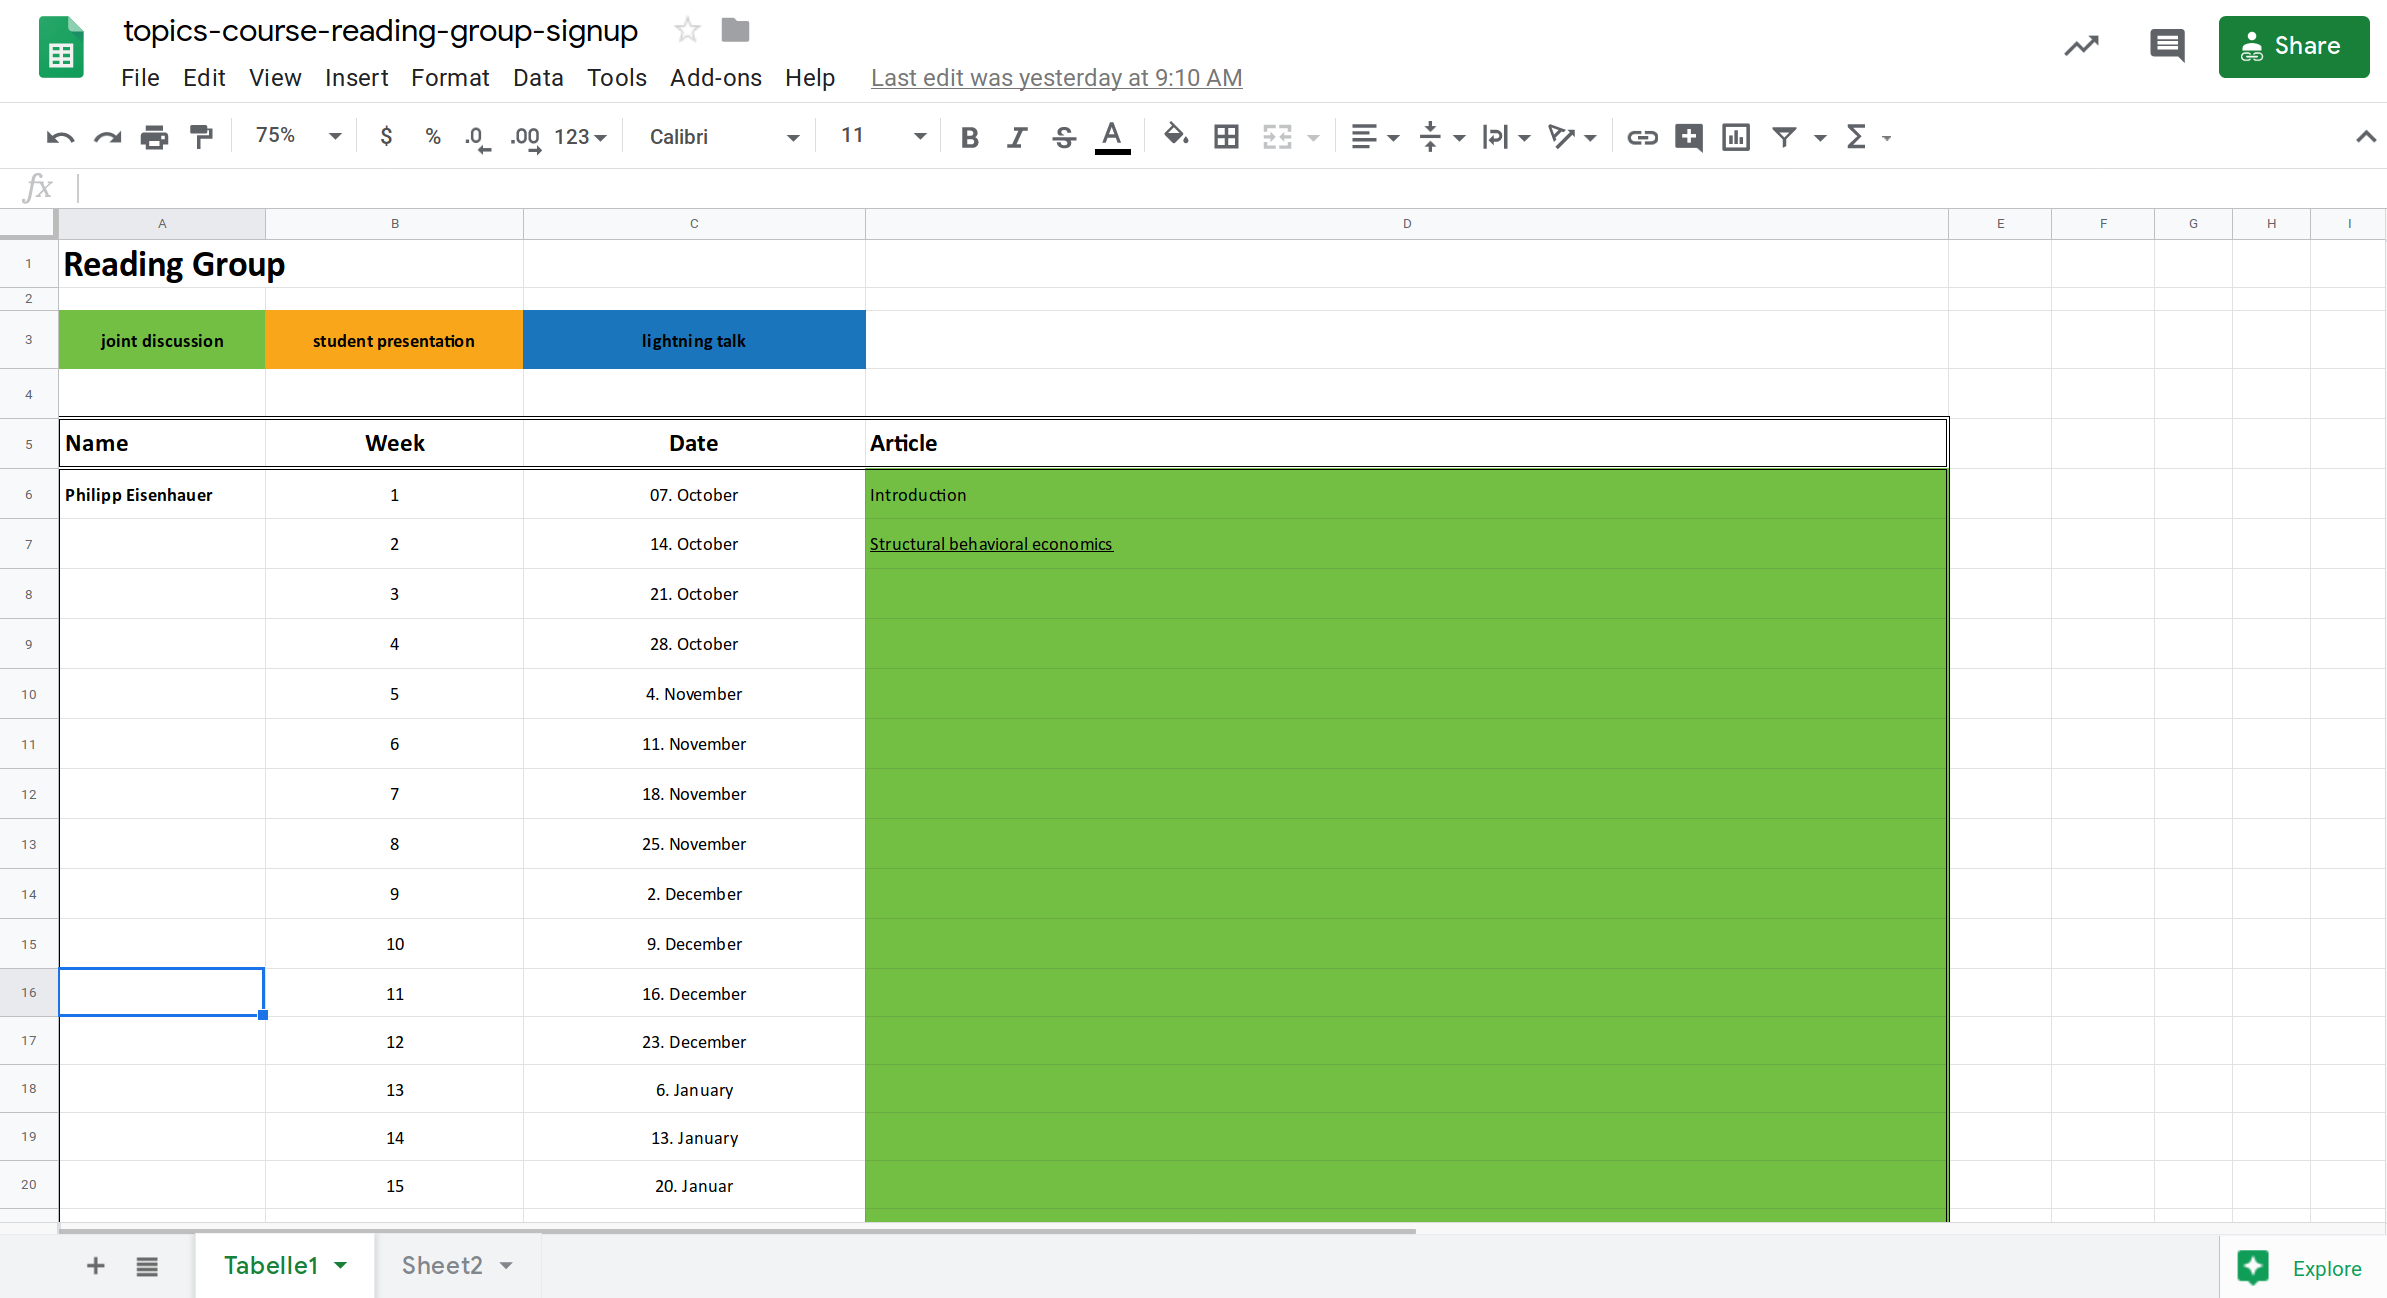
\includegraphics{fig-reading-group-signup}}
\end{figure}
\end{frame}
%-------------------------------------------------------------------------------
%-------------------------------------------------------------------------------
\begin{frame}\textbf{Tooling}\vspace{0.5cm}
\begin{columns}[t]
	\column{.5\textwidth}
	\centering \\
	% Python
	
\includegraphics[width=0.6\textwidth]{fig-tooling-python.png}\\
	\vspace{1.5cm}
	% GitHub
	
\includegraphics[width=0.45\textwidth]{fig-tooling-github.png} \\
	\vspace{-0.5cm}
	\column{.5\textwidth}
	\centering \\
	% Scipy
	
\includegraphics[width=0.6\textwidth]{fig-tooling-scipy.png} \\
	\vspace{1cm}
	% Jupyter
	
\includegraphics[width=0.45\textwidth]{fig-tooling-jupyter.png} \\
	\vspace{-0.2cm}
\end{columns}
\end{frame}
%-------------------------------------------------------------------------------
%-------------------------------------------------------------------------------
\begin{frame}\textbf{OpenSourceEconomics}\vspace{0.5cm}

\begin{center}\begin{quote}
We are a group of economists using computational models in the pursuit of our research. By adopting sound software engineering practices, we hope to leverage tools from computational science and increase the transparency and extensibility of our implementations. In doing so, we expand the set of possible economic questions that we can address and improve the quality of our answers.
\end{quote}\end{center}
\end{frame}
%-------------------------------------------------------------------------------
%-------------------------------------------------------------------------------
\begin{frame}[c]
\begin{figure}
\scalebox{0.2}{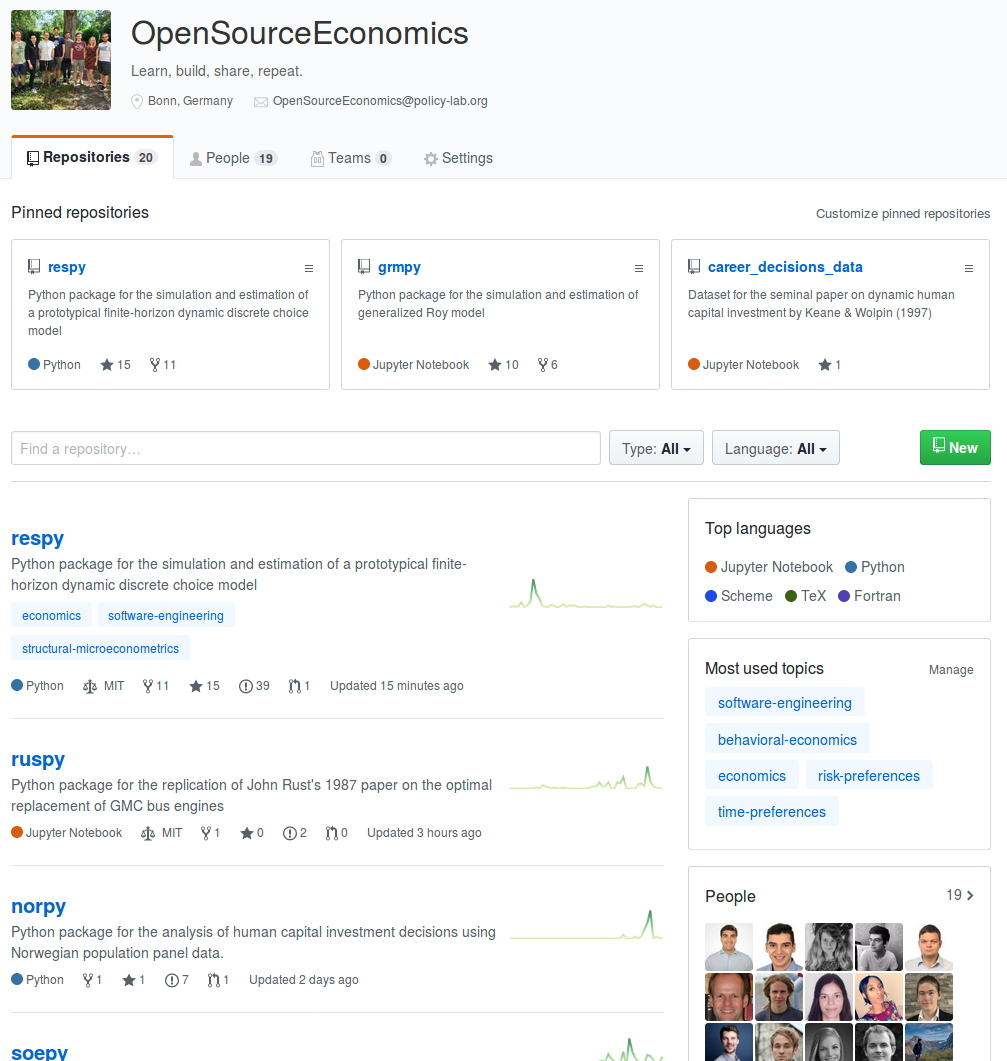
\includegraphics{fig-ose-github}}
\end{figure}
\end{frame}
%-------------------------------------------------------------------------------
%-------------------------------------------------------------------------------
\begin{frame}
\textbf{Communication}\\\vspace{0.5cm}
\begin{tabular}{ll}
Slack     & \url{http://bit.ly/human-capital-slack} \\
          & \url{http://bit.ly/ose-slack} \\
          &                                          \\
GitHub    & \url{http://bit.ly/human-capital-github} \\
          & \url{http://bit.ly/ose-github} \\
\end{tabular}
\end{frame}
%-------------------------------------------------------------------------------
%-------------------------------------------------------------------------------
\begin{frame}
\begin{figure}[htp]\centering
\caption{Communications}
\scalebox{0.125}{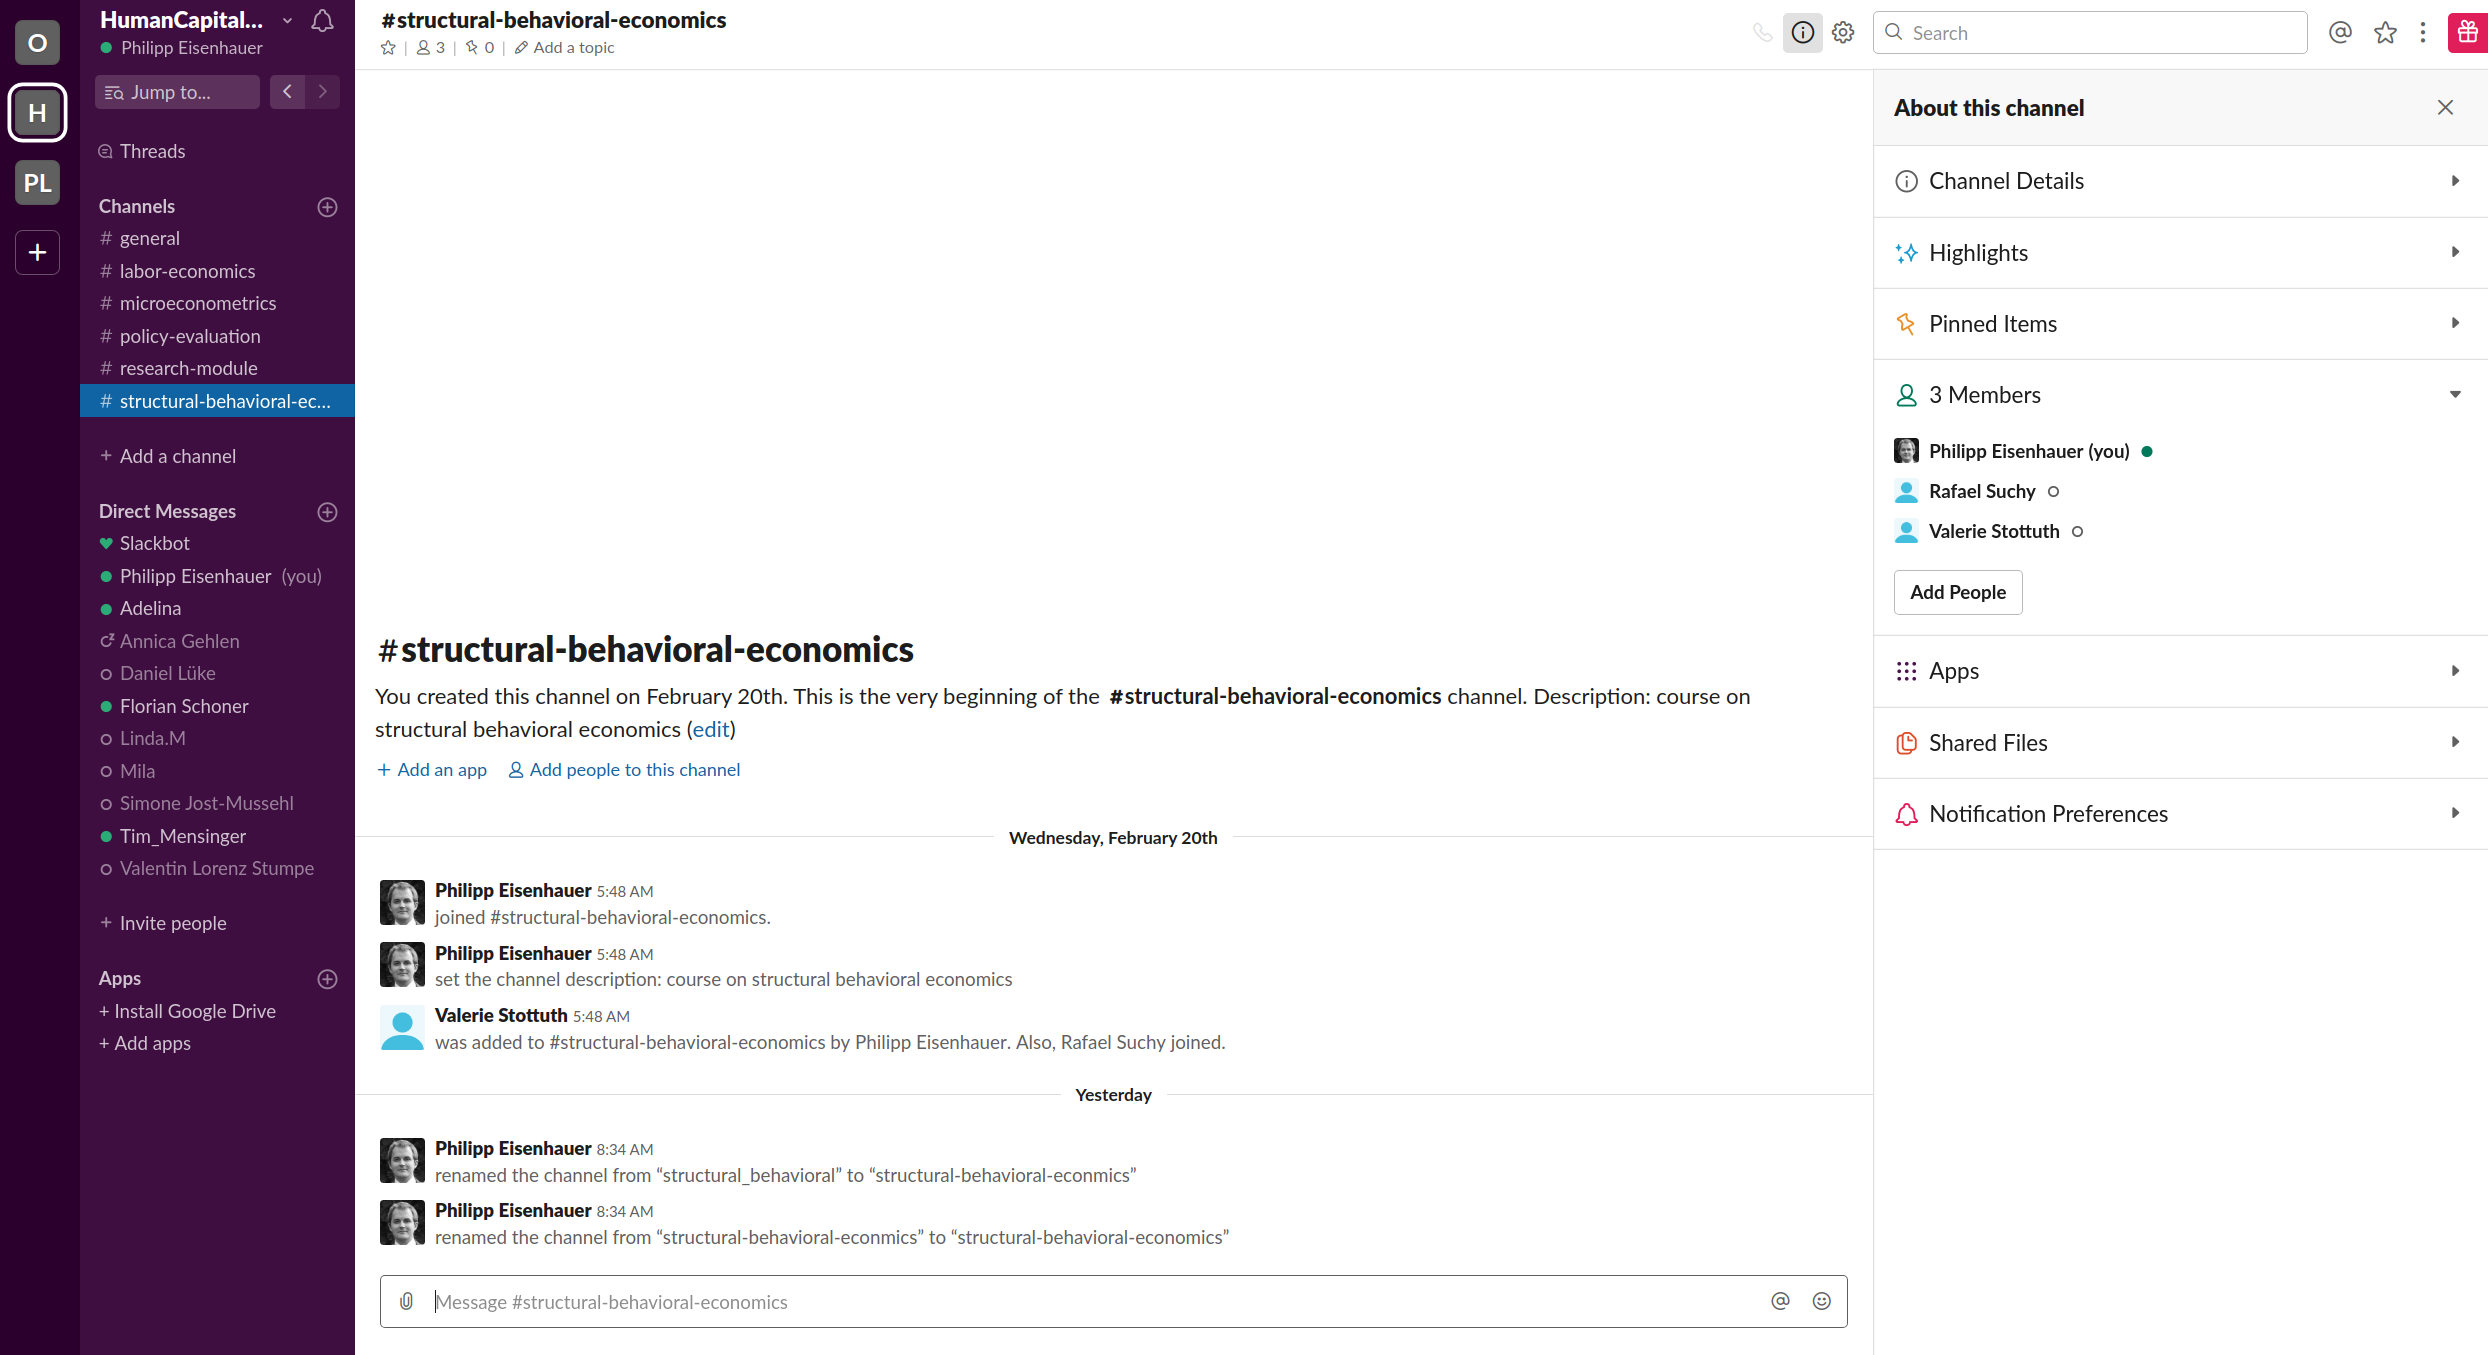
\includegraphics{fig-reading-group-slack}}
\end{figure}
\end{frame}
%-------------------------------------------------------------------------------
%-------------------------------------------------------------------------------
\begin{frame}\textbf{Common baseline}\vspace{0.5cm}

\begin{itemize}\setlength\itemsep{1em}
\item \bibentry{Keane.1997}
\item \bibentry{respy-1.0}
\end{itemize}

\end{frame}
%-------------------------------------------------------------------------------
%-------------------------------------------------------------------------------
\begin{frame}
\begin{figure}[htp]\centering
\caption{Code documentation}
\scalebox{0.15}{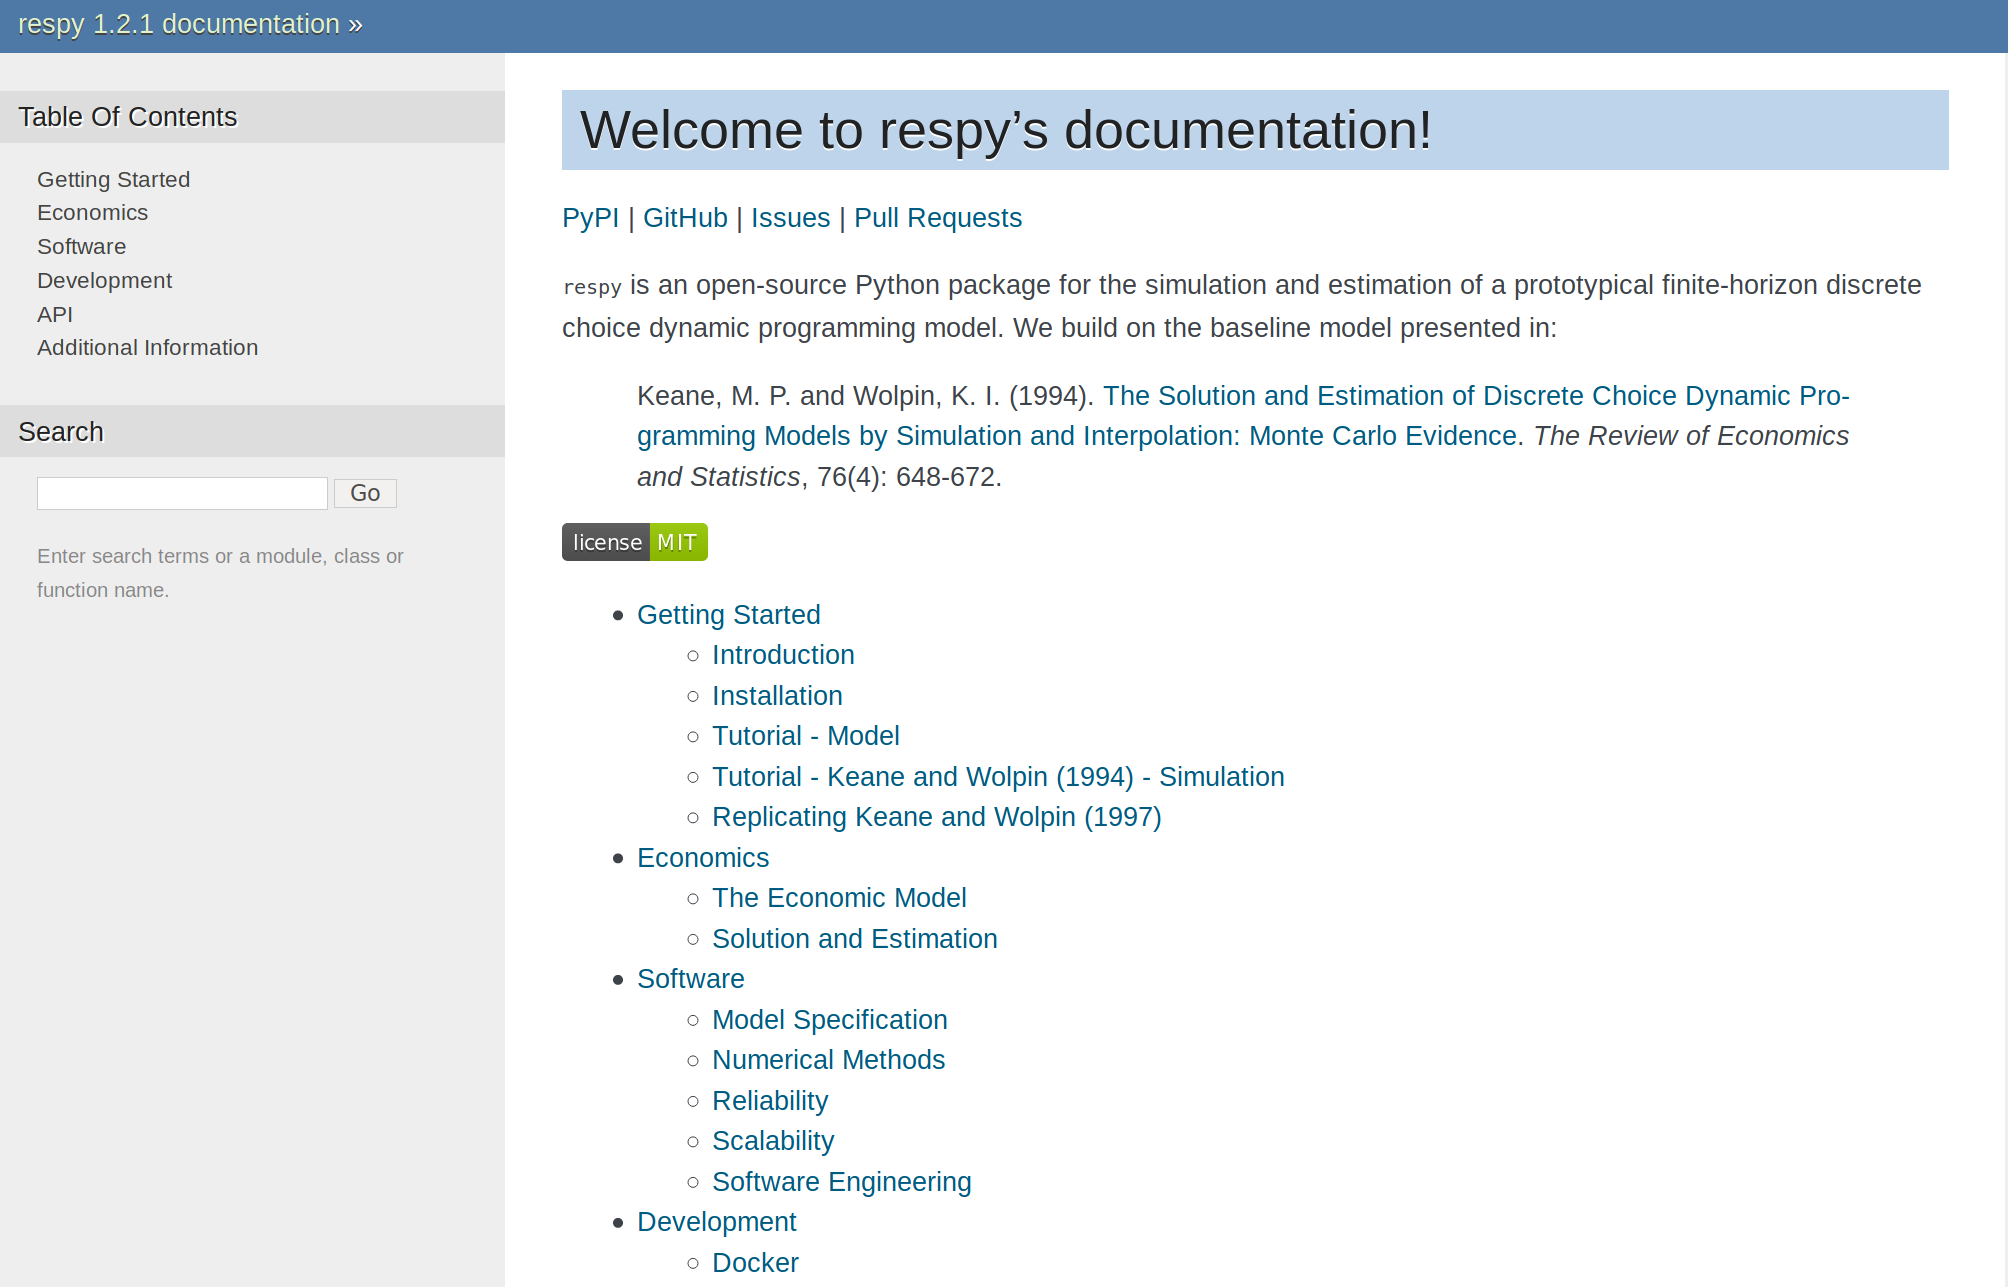
\includegraphics{fig-respy-documentation}}
\end{figure}
\end{frame}
%-------------------------------------------------------------------------------
%-------------------------------------------------------------------------------
\begin{frame}\textbf{Behavioral structural econometrics}\vspace{0.5cm}

\begin{itemize}\setlength\itemsep{1em}
\item \bibentry{DellaVigna.2018}
\end{itemize}

\end{frame}
%-------------------------------------------------------------------------------
%-------------------------------------------------------------------------------
\begin{frame}\begin{center}
\LARGE\textbf{Student project}
\end{center}\end{frame}
%-------------------------------------------------------------------------------
%-------------------------------------------------------------------------------
\begin{frame}\begin{center}
\LARGE\textbf{Conclusion}
\end{center}\end{frame}
